\clearpage
\appendix
\section{Failure Mechanisms and Design Disposition}
\label{sec:failure-map}
\label{sec:design-summary}
\begin{table}[htbp]
\centering\small
\caption{What failed, the observed mechanism and the resulting engineering decision.}
\begin{tabularx}{\linewidth}{@{}L{0.19\linewidth}Y Y@{}}
\toprule Design / evidence & Failure mechanism & Disposition and remaining limit \\\midrule
Any-hit evidence gate; factual confirmation & The generator expected one or two selected claims; the gate passed an unrestricted set. Correct retrieval therefore ended in abstention. & Preserve as a failed interface control. Use question-targeted selection and ambiguity checks; 63.25\% still fails complete-answer acceptance. \\
Dense/hybrid retrieval; same factual set & Higher complexity did not improve downstream scores: 62\% versus BM25's 63.25\%.  & Retain BM25 locally.  \\
Visual retrieval; omni confirmation & Candidate failures concentrated in packet layouts and source-region attribution: 16/30 grounded and 16/30 original-region lineage. & Drop this candidate. The 26/30 text/OCR control also had a wrong-region/invalid citation; visual capability remains limited. \\
Instruction and revision; fresh paired drafts & Source-linked wording could assert sufficiency from a necessary condition. Both revision candidates preserved 56/56 drafts and repaired 47/56, but each retained one critical failure. & Do not promote based on aggregate repair rate. Validate the delivered claims, including supplementary examples. \\
Learner assessment; multi-concept correction & One assessment spread across weak concept matches. Primary-concept-only assignment corrected that attribution problem. & Keep concept-assessment correction. The later goal audit found 10 unsupported completions in this historical run; the new paired lifecycle study removes that defect. Prediction and teaching remain separate. \\
Goal completion; the \hyperref[study-H]{goal-completion regression} & The strongest concept's evidence completed unrelated goals. Both the service shortcut and interpreter lacked target-specific binding. & Require every concept of the exact objective. Unsupported completions fell from 12 to zero; mean final simulator mastery changed by $-0.0024$ relative to the old logic. \\
Model-backed outreach; saved dialogue & All 16 reviewed check-ins wrapped an entire source card in generic guidance. Permission checks did not assess instructional usefulness. & Retain operational evidence only; contextual progression needs separate evaluation. \\
Evaluation oracle; corrected controls & A source/reference packet reversed a one-way implication; structural checks did not detect every semantic defect. & Preserve invalid and corrected records. AI review is diagnostic; quality claims need independently checked reference meaning. \\
\bottomrule
\end{tabularx}
\end{table}

The linked evidence index in Appendix~\ref{sec:study-index} identifies the
source records. Historical attempts remain in the repository, including
invalid results and subsequent corrections. \clearpage
\section{Publication and Data Relationships}
\label{sec:publication-data}
Figure~\ref{fig:data-detail} identifies the persistent relationships used by
publication and tutoring.
\begingroup
\setlength{\intextsep}{3pt}
\setlength{\abovecaptionskip}{4pt}
\begin{figure}[!ht]
\centering
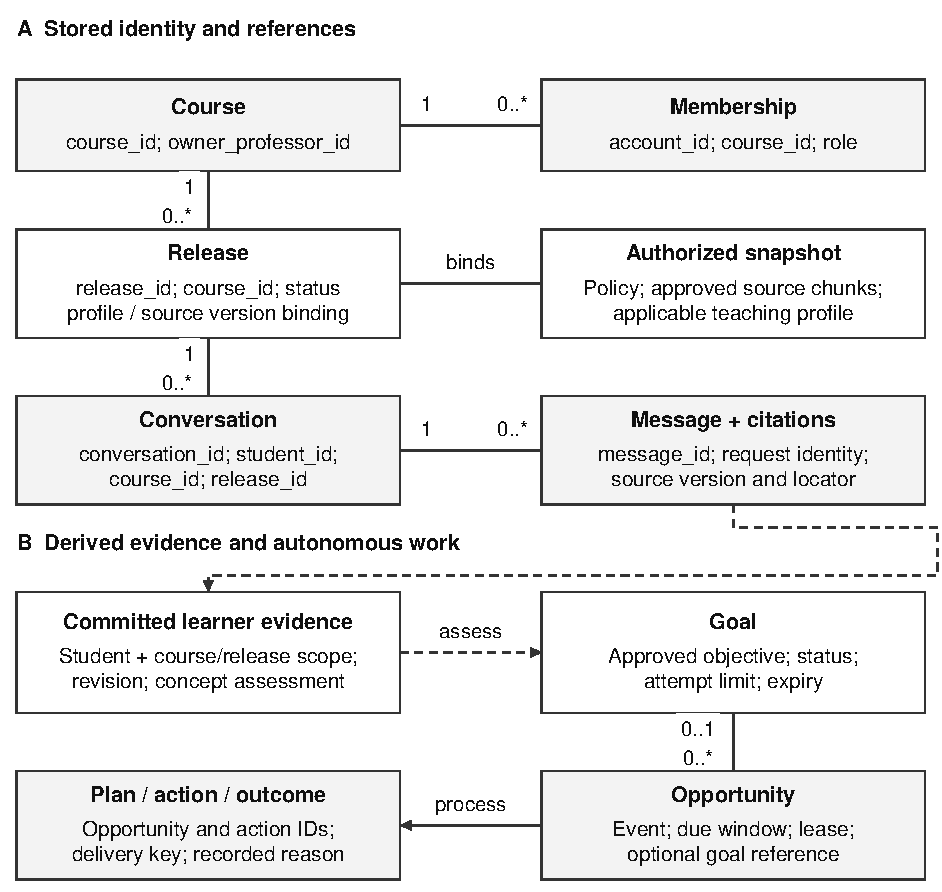
\includegraphics[width=\linewidth]{../../../reports/figures/course-twin-data-relationships.pdf}
\caption{Conceptual relationships among course releases, conversations, learner evidence and autonomous work.}
\label{fig:data-detail}
\end{figure}
\FloatBarrier
\endgroup
\clearpage
Publication is a separate state transition from preview or preflight.
Figure~\ref{fig:publication-detail} shows both operations and their failure
boundary. The preflight records deterministic readiness checks; it does not
replace the academic quality evaluations in the results section. The observer
runs after publication commits. Rollback revalidates and republishes a withdrawn release.
\begin{figure}[!ht]
\centering
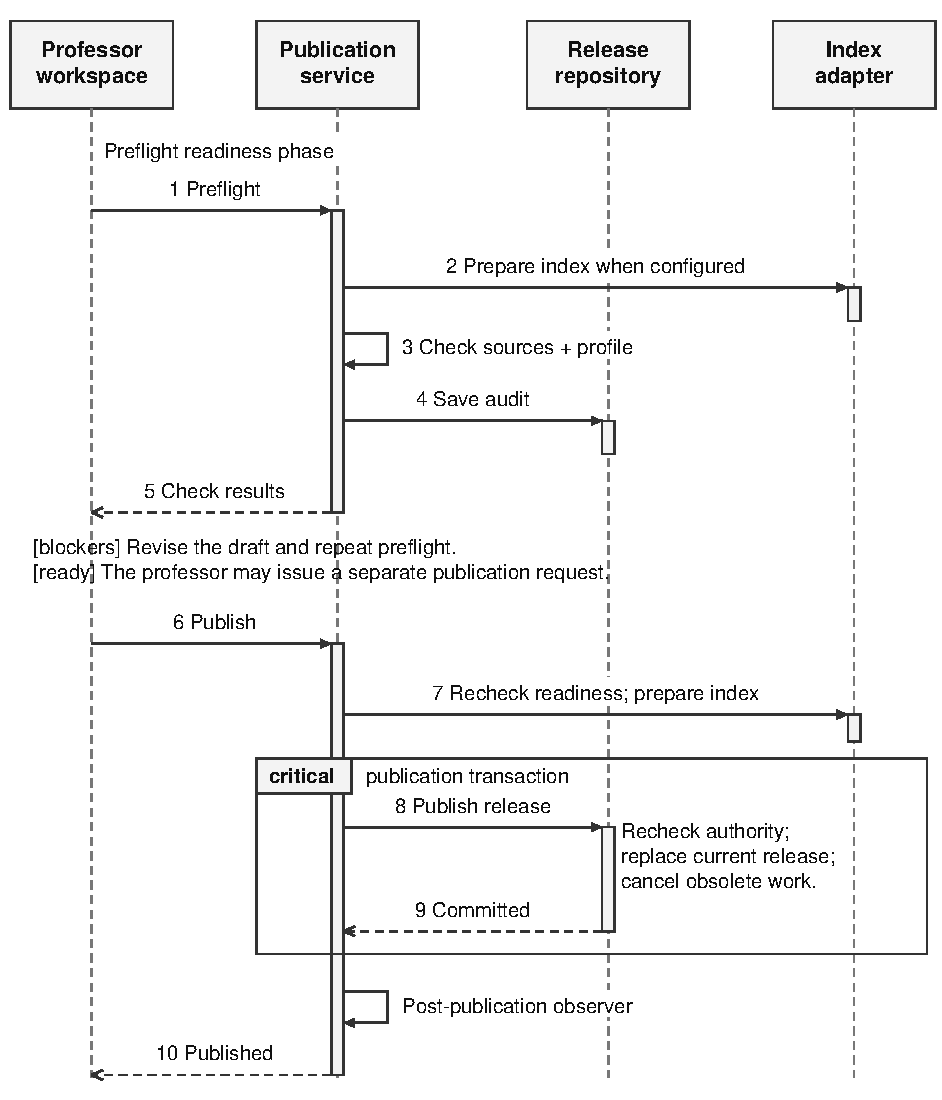
\includegraphics[width=\linewidth]{../../../reports/figures/course-twin-publication-sequence.pdf}
\caption{Preflight and publication interactions, with the release transaction shown explicitly.}
\label{fig:publication-detail}
\end{figure}
\FloatBarrier

\clearpage
\section{Software and Reproducibility}
\label{sec:software}
The retained component profile is
\path{research/05_evaluation/profiles/student-tutor-r1-local-final-v1.json}.
The project repository is \url{https://github.com/horiiiiii032929/digital-twin}
\cite{horinouchi2026digitaltwin}. It contains source code, synthetic evaluation
instruments and durable result summaries. Sensitive material and bulky generated
outputs are excluded. A repository URL identifies the project, not an immutable
experimental snapshot: reproduce a result using its recorded source revision,
dirty-state manifest, model configuration and dataset identifiers.

Table~\ref{tab:software} links the principal implementation dependencies to their
official documentation. Versions are taken from the current \path{uv.lock} and
\path{package-lock.json}, inspected on 6 September 2026; they are not attributed
to every historical run. Dynamic documentation was accessed on the same date.
Optional retrieval packages support comparisons and are not all selected runtime
components. The Qwen3 reranker adapter uses the prompt template published in the
\href{https://huggingface.co/Qwen/Qwen3-Reranker-0.6B}{Qwen3-Reranker model card};
that template is not a project contribution. 

\begin{table}[htbp]
\centering\small
\caption{Principal software dependencies (locked versions).}
\label{tab:software}
\begin{tabularx}{\linewidth}{@{}>{\raggedright\arraybackslash}L{0.22\linewidth}>{\raggedright\arraybackslash}Y@{}}
\toprule
Role & Software and official documentation \\
\midrule
API and validation & \href{https://fastapi.tiangolo.com/}{FastAPI} (0.141.1), \href{https://pydantic.dev/docs/validation/latest/get-started/}{Pydantic} (2.13.4). \\
Workflow and state & \href{https://docs.langchain.com/oss/python/langgraph/overview}{LangGraph} (1.2.11), SQLite checkpoint package (3.1.1), \href{https://www.sqlite.org/docs.html}{SQLite}, \href{https://aiosqlite.omnilib.dev/en/stable/}{aiosqlite} (0.22.1). \\
Model transport & \href{https://docs.litellm.ai/docs/}{LiteLLM} (1.97.0), \href{https://www.python-httpx.org/}{HTTPX} (0.28.1), \href{https://developers.openai.com/api/docs/guides/text}{OpenAI Responses API}. \\
Document processing & \href{https://pymupdf.readthedocs.io/en/latest/}{PyMuPDF} (1.28.2). \\
Web application & \href{https://react.dev/}{React} (19.2.8), \href{https://www.typescriptlang.org/docs/}{TypeScript} (7.0.2), \href{https://vite.dev/guide/}{Vite} (8.2.1), \href{https://tailwindcss.com/docs/installation/using-vite}{Tailwind CSS} (4.3.3). \\
Optional retrieval & \href{https://huggingface.co/docs/transformers/index}{Transformers} (5.15.1), \href{https://docs.pytorch.org/docs/stable/index.html}{PyTorch} (2.13.0), \href{https://www.sbert.net/}{Sentence Transformers} (6.0.0), \href{https://qdrant.github.io/fastembed/}{FastEmbed} (0.8.0). \\
Deployment & \href{https://docs.docker.com/compose/}{Docker Compose}, \href{https://caddyserver.com/docs/}{Caddy}; image configuration is recorded in the deployment files. \\
Testing & \href{https://docs.pytest.org/en/stable/}{pytest} (9.1.1), \href{https://vitest.dev/guide/}{Vitest} (4.1.10). \\
Dependency and report builds & \href{https://docs.astral.sh/uv/}{uv}, \href{https://tectonic-typesetting.github.io/en-US/}{Tectonic}, \href{https://ctan.org/pkg/natbib}{natbib}. \\
\bottomrule
\end{tabularx}
\end{table}

Diagram preparation was informed by Lek Hsiang Hui's IT5004 lectures 4,
``Requirements Analysis'' (PDF pp. 10--20, 54--58), and 5, ``Introduction to
Enterprise System'' (PDF pp. 7--19, 24--29), supplied as course materials;
the figures depict this project's implementation.

The repository README documents \verb|uv sync --locked --dev|,
\texttt{npm ci} and \texttt{npm run check}. The report README records the
Tectonic build command. Model identifiers and experimental selections are
versioned separately from library dependencies. 


\clearpage
\section{Development Lifecycle Traceability}
\label{sec:sdlc}
\begin{table}[htbp]
\centering\small
\caption{SDLC artifacts and acceptance conditions.}
\label{tab:sdlc}
\begin{tabularx}{\linewidth}{@{}L{0.17\linewidth}Y Y@{}}
\toprule Stage & Retained artifact and responsibility & Acceptance and next step \\\midrule
Requirements & Five user requirements in Table~\ref{tab:requirements}; approved project brief; \path{docs/quality-and-learning-plan.md}. Instructor defines knowledge, teaching policy and publication authority. & Walkthrough explains intended behaviour; instructor fidelity and real-course acceptance still require review. \\
Design & Architecture, response sequence and autonomy activity; \path{research/05_evaluation/profiles/}. Interfaces separate policy, providers and persistence. & Compare alternatives under shared conditions; retain unsuccessful choices and explicit fallback. \\
Implementation & Domain logic in \path{src/}, API in \path{services/}, interface in \path{apps/}; locked dependencies. & Trace requirements to executable boundaries; use \texttt{npm run check} for application checks.  \\
Verification & \path{tests/}; versioned cases and \path{research/05_evaluation/result-registry.md}. & Factual-support and teaching-alignment gates remain unresolved. Continuing-support simulations assess continuity under artificial events, not student learning. \\
Deployment & \path{docs/local-r1-runbook.md}; qualified configuration and rollback control. Operator starts API and workers with a shared persistent store. & Local qualification has a bounded environment. Confirm the exact profile, restore procedure and access controls before each deployment. \\
Operation and revision & Persisted goals, actions, outcomes and audit events; instructor dashboard and publication controls. & Observe failures, pause/withdraw when required, reproduce a defect, revise a candidate and rerun affected checks before updating the selected profile. \\
\bottomrule
\end{tabularx}
\end{table}

The goal-completion repair passed 72 focused service, component and audit tests.
The broader Python run and targeted rechecks verified 2,600 distinct tests;
this was not a single clean full-suite run after correction. The linked
\hyperref[study-H]{goal-completion record} preserves the initial failures,
local HTTPS permission issue, evaluation-runner classification repair and JUnit
records. The historical autonomy example is traced separately in
Appendix~\ref{sec:historical-autonomy}.

\clearpage
\section{Evidence Index}\label{sec:study-index}
Each link below opens the durable result summary, which records the configuration,
case counts, decision and limitations. The repository retains the full result
registry and individual attempts; raw execution settings, repeated approvals and
plan inventories are not reproduced in this report.
\begin{longtable}{@{}L{0.38\linewidth}L{0.57\linewidth}@{}}
\toprule Comparison & Evidence record \\ \midrule
\endhead
\phantomsection\label{study-A}Evidence-interface comparison & \href{https://github.com/horiiiiii032929/digital-twin/blob/main/research/05_evaluation/course-digital-twin-whole-system-architecture-round-2-001-results.md}{Result, method and limitations} \\
\phantomsection\label{study-B}Fresh factual comparison & \href{https://github.com/horiiiiii032929/digital-twin/blob/main/research/05_evaluation/final-cross-method-factual-confirmation-001-results.md}{Result, method and limitations} \\
\phantomsection\label{study-C}Action-planning comparison & \href{https://github.com/horiiiiii032929/digital-twin/blob/main/research/05_evaluation/successor-architecture-confirmation-005-001-results.md}{Result, method and limitations} \\
\phantomsection\label{study-D}Model-allocation comparison & \href{https://github.com/horiiiiii032929/digital-twin/blob/main/research/05_evaluation/successor-architecture-engine-comparison-006-001-results.md}{Result, method and limitations} \\
\phantomsection\label{study-E}Learner/timing simulation & \href{https://github.com/horiiiiii032929/digital-twin/blob/main/research/05_evaluation/successor-learner-timing-simulation-001-results.md}{Result, method and limitations} \\
\phantomsection\label{study-F}Revision comparison & \href{https://github.com/horiiiiii032929/digital-twin/blob/main/research/05_evaluation/independent-factual-revision-controls-001-fresh-v16-live-001-results.md}{Result, method and limitations} \\
\phantomsection\label{study-G}Live-model integration trial & \href{https://github.com/horiiiiii032929/digital-twin/blob/main/research/05_evaluation/final-profile-operational-dialogue-development-001-full-live-001-results.md}{Result, method and limitations} \\
\phantomsection\label{study-H}Goal-completion regression & \href{https://github.com/horiiiiii032929/digital-twin/blob/main/research/05_evaluation/goal-completion-scope-development-001-results.md}{Result, method and limitations} \\
\phantomsection\label{study-L1}Pipeline-scale test & \href{https://github.com/horiiiiii032929/digital-twin/blob/main/research/05_evaluation/factual-qa-v3-scale-completion-10000-001-results.md}{Result, method and limitations} \\
\phantomsection\label{study-L1c}Pipeline-test correction & \href{https://github.com/horiiiiii032929/digital-twin/blob/main/research/05_evaluation/factual-qa-v3-scale-completion-10000-001-analysis-correction-001-results.md}{Result, method and limitations} \\
\phantomsection\label{study-L2}Large product test & \href{https://github.com/horiiiiii032929/digital-twin/blob/main/research/05_evaluation/course-digital-twin-evaluation-program-011-results.md}{Result, method and limitations} \\
\phantomsection\label{study-L3}Whole-corpus regression & \href{https://github.com/horiiiiii032929/digital-twin/blob/main/research/05_evaluation/academic-factual-qa-open-10000-winner-regression-001-results.md}{Result, method and limitations} \\
\bottomrule\end{longtable}
The pipeline correction supersedes the original quality interpretation; neither
record is deleted. The goal-completion record compares old and corrected logic
and links the two arms. Its \href{https://github.com/horiiiiii032929/digital-twin/blob/main/research/05_evaluation/goal-completion-scope-review-audit-001-results.md}{scope audit}
explains the historical correction. The whole-corpus result contains the unresolved
numerical inconsistency discussed in Section~\ref{sec:large-regression}; its
headline percentage is not used as validated performance evidence.

\clearpage
\section{Planner Calculation and Evaluation Definitions}
\label{sec:planner-math}
This appendix expands the executable heuristic in
\path{src/digital_twin/student/planning_architectures.py}.
It describes the inspected implementation, not fitted educational parameters.
For an action $a$, let $p$ be the planning probability proxy, $u$ its uncertainty,
$z$ goal progress and $L$ the look-ahead depth (default two). With elapsed
observation time $t$ in days, spacing is $s=1-\exp(-t/3)$; when $t$ is absent,
the implementation uses $s=1$. The default adapter leaves $t$ absent.

\begin{align}
G(a)&=\min\{1,\ g_a(1-p)(0.5+0.5s)\},\\
O(a)&=\min\{1,\ o_a(0.5+0.5u)\},\\
F(a)&=\min\{1,\ 0.35L[G(a)+O(a)](1-z)\}.
\end{align}
The misconception bonus is $0.12$ for a hint/example or $0.04$ for a diagnostic
question when the inferred incorrect streak is at least two, otherwise zero.
Evidence risk is one when evidence is not ready, otherwise zero, with an
additional $0.05\max(0,k-2)$ for a check-in and clipping at one. Here $k$ is
the state card's evidence count; the default adapter populates it with the
number of supporting observation identifiers. The guarded
planner returns no action before scoring when its evidence-readiness check
fails; the risk term remains part of the shared forward-model interface.
No action has all terms and utility equal to zero.

\begin{table}[htbp]
\centering\small
\caption{Action constants used by the analytic forward model. Only
event-eligible and instructor-permitted actions are scored for a job.}
\begin{tabularx}{\linewidth}{@{}Yrrr@{}}
\toprule Action & $g_a$ & $o_a$ & $I(a)$ \\\midrule
Diagnostic question & 0.05 & 0.28 & 0.03 \\
Hint or example & 0.18 & 0.12 & 0.04 \\
Approved-source recommendation & 0.12 & 0.08 & 0.04 \\
Retrieval practice & 0.24 & 0.24 & 0.05 \\
Schedule follow-up & 0.02 & 0.03 & 0.02 \\
In-app check-in & 0.03 & 0.05 & 0.08 \\
Progress summary & 0.04 & 0.02 & 0.04 \\
Professor insight draft & 0.01 & 0.00 & 0.01 \\
No action & 0.00 & 0.00 & 0.00 \\
\bottomrule
\end{tabularx}
\end{table}

For the worked calculation in Section~\ref{sec:planning}, a hint has
$G=0.09$, $O=0.08$, $F=0.119$, $B=0.12$, $R=0$ and $I=0.04$.
The sum is $0.325$. The diagnostic question has $G=0.025$,
$O\approx0.186667$, $F\approx0.148167$, $B=0.04$, $R=0$ and $I=0.03$,
giving approximately $0.267167$. This is a calculation from constants and a
declared state, not an invented empirical case.

The component evaluation uses a different quantity. If the hidden instrument
assigns action value $v_i(a)$ in context $i$, the selected action is $\hat a_i$
and $N$ is the number of contexts, then
\begin{equation}
\overline v=\frac1N\sum_i v_i(\hat a_i),\qquad
\overline r=\frac1N\sum_i\left[\max_a v_i(a)-v_i(\hat a_i)\right].
\end{equation}
The \hyperref[study-C]{action-planning comparison}'s utility improvement is $0.004805$, with paired 95\% interval
$0.003065$--$0.006760$ over 1,000 contexts. Its preferred-label difference
is $-0.01$, with interval $-0.022$--$0.001$. Utility, preferred action and
the runtime score therefore answer different questions. The synthetic action
values and the model's internal prediction do not constitute observed learning.

\clearpage
\section{Synthetic Teaching Profiles and Saved Responses}\label{sec:profile-examples}
A teaching profile specifies tone, explanation depth, examples, misconception
handling and the sequence of assistance. A Socratic policy can prefer an initial
question or a hint; an explanatory policy can permit a direct explanation.
The synthetic profiles used in the saved dialogue trial expose eight fields
(Table~\ref{tab:profile-fields}). Their values enter the approved teaching-context
candidate, where the service supplies them together with the current question,
permitted evidence and dialogue state. A profile change therefore needs a new
reviewed binding; a student message is not allowed to replace that configuration.

\begin{table}[htbp]
\centering\small
\caption{Teaching fields in the live-model integration trial's synthetic profiles.}
\label{tab:profile-fields}
\begin{tabularx}{\linewidth}{@{}L{0.24\linewidth}YY@{}}
\toprule Field & Socratic configuration & Explanatory configuration \\\midrule
Tone / depth & Patient and reflective; concise & Direct and precise; detailed \\
Explanation structure & Diagnostic question, attempt, one hint & Explanation, example, understanding check \\
Example preference & Learner constructs an example & Concrete non-assessed example \\
Misconception handling & Contrast question before correction & Explain correction, then apply it \\
Integrity limits & Require an attempt; no assessed-work solutions & Same restriction \\
Help ladder & Question, hint, guided explanation & Explanation, worked example, application question \\
Outreach policy & Reflective lead; contrast alternatives & Direct lead; apply the evidence \\
\bottomrule
\end{tabularx}
\end{table}
Source: \path{scripts/teaching_profile_responsiveness_packet.py}, used by the
operational dialogue runner. Tone and depth are separate fields shown together
for compactness. 

Table~\ref{tab:worked-example} uses saved outputs from the 24-history operational
trial. These are separate synthetic contexts, not a controlled comparison of the
effect of changing a single profile.

\begin{table}[htbp]
\centering\small
\caption{Saved configuration-to-response examples from the live-model integration trial.}
\label{tab:worked-example}
\begin{tabularx}{\linewidth}{@{}L{0.20\linewidth}Y@{}}
\toprule Context & Stored output and interpretation \\\midrule
Socratic; first turn & Student: ``How does slot seal work in this course protocol?'' Tutor: ``For `How does slot seal work', what is your current explanation, and which step are you unsure about?'' The system elicits an attempt, but the question remains generic. \\
Explanatory; day 30 & Student asks how lantern check works. Tutor: ``lantern check sends a probe to each station'' and ``marks a station unavailable after two consecutive unanswered probes''. The reply supplies the source rule; repeated extraction does not establish personalized progression. \\
Proactive support & All 16 reviewed check-ins used a generic wrapper around an entire synthetic source card. Authority checks permitted delivery; the effect of these messages on students was not measured. \\
\bottomrule
\end{tabularx}
\end{table}
The source record is \path{research/05_evaluation/dialogue-full-live-001-assistant-findings.json};
its finding identifiers F21 (Socratic example) and F03 (explanatory example) retain the history, day, student input, response and diagnostic finding.
The operational trial is reported in Section~\ref{sec:provider-study} and indexed
in Appendix~\ref{sec:study-index}.


\clearpage
\section{Historical Multi-concept Trial and Correction}\label{sec:historical-autonomy}
\textbf{Recorded example.} In the saved deterministic fast-learner history
(seed 3101, Bayesian-style simulator), the first day contains a diagnostic
question and a hint. Before the next recorded student turn, an
\texttt{incomplete-objective} event produces an in-app check-in: the goal still
requires assessed evidence, and the deterministic event rule selects that
permitted action. The saved opportunity, action and delivery-message identifiers
link the decision to its persisted effect and source citation. Subsequent turns
produce further learner-state revisions; the day-15 restart check retains an
identical state hash. By the end, the token-bucket concept has eight correct and
four incorrect assessments, illustrating why a delivered check-in is not itself
proof of mastery. This is one operational trace, not evidence that the check-in
caused those later outcomes. Its source is the \href{https://github.com/horiiiiii032929/digital-twin/blob/main/research/05_evaluation/governed-full-autonomy-v2-1-multi-concept-confirmation-025-results.md}{historical multi-concept result}; the sanitized trace is retained in
\path{research/06_reports/final/professor-reader-review.md}.


\subsection{Original Reported Simulator Outcomes}
For the autonomous-support question, the deterministic longitudinal study compared 72 histories in 36 matched pairs.
A pair shares the specified learner scenario and seed, with autonomous support
in one history and reactive-only support in the other. This is a comparison
within the simulator, not a randomized study of students.
It exercised 30 virtual days of tutoring and intervention logic without external
LLM calls. Simulated mastery averaged 0.365 with autonomous support and 0.332
with the reactive control; the paired difference was 0.0324, with a 95\% interval
of 0.0040--0.0617. For pair $k$, let $m_k^{A}$ and $m_k^{R}$ be final simulated mastery under
autonomous and reactive support, respectively. Each history's mastery summarizes
its simulated concepts on a zero-to-one scale. The paired mean difference is
\begin{equation}
\overline{\Delta m}=\frac{1}{36}\sum_{k=1}^{36}(m_k^{A}-m_k^{R})=0.0324.
\label{eq:mastery-difference}
\end{equation}
This is 3.24 percentage points on the simulator's scale. It is computed from
unrounded paired values, so subtracting the displayed rounded means need not
reproduce it exactly. Its interval resamples the paired differences. Both the
means and their difference follow the simulator's learning and forgetting rules;
they are not measured student learning gains.

Predictive area under the receiver operating characteristic curve (AUROC) summarizes how well the previous learner-state estimate ranks
later correct above incorrect simulated attempts. A value of 0.5 gives no ranking
advantage; 1 indicates perfect ranking. The reported 0.466, averaged over histories with both outcomes, therefore
provides little evidence of useful prediction. A simulated intervention is labelled
wasted when its recipient is already at the mastery threshold or is unreceptive.
The reported 32.9\% is an average of per-history wasted-delivery rates, rather
than a human judgment of whether a message helped. These diagnostics reveal
weaknesses that successful consent and restart checks cannot detect.


\paragraph{Later interpretation correction.}
These numbers describe the original multi-concept implementation. The subsequent
goal-scope audit found ten unsupported completed goals among 22 completions
across eight histories, even though the concept-assessment gates had passed.
The old paired mastery difference is therefore retained as a historical
simulator outcome, not evidence for the corrected lifecycle or real learning.
The \hyperref[study-H]{goal-completion regression} uses new seeds on the same exposed concepts and reports its own
paired results; it does not overwrite or rescore the historical trial.




